\section{Discussion}
\label{ch:discussion}

\subsection{Relation to Empirical Evidence}

The argument of this paper does not depend on experiments, but the symptoms of Mode B have long been recorded extensively in the empirical literature, and a comparison is worthwhile. Deep networks can memorize random labels with near-zero training error, showing that frozen weights suffice to hold the numerical table of an entire corpus \citep{zhang2021}; shortcut learning shows that what networks preferentially learn are the effort-saving statistical correlations in the corpus rather than the structure the task requires \citep{geirhos2020}; on out-of-distribution inputs, confidence is distorted and dedicated detection baselines are needed \citep{hendrycks2016}, later developed into a systematic spectrum of detection methods \citep{yang2024}, and high-confidence responses can be induced by stimuli dissimilar to any natural input \citep{nguyen2014}. These observations corroborate the same fact from three sides, namely memory capacity, learning preference, and out-of-distribution behavior: what frozen parameters carry are the statistics of a corpus, not rules generated from current evidence. The causal direction must be emphasized: this paper does not induce its conclusion from these phenomena but deduces it from the defining features of the task; the empirical phenomena are merely projections of the deductive conclusion into the laboratory.

\subsection{A Minimal Empirical Probe of the Risk Gap}
\label{sec:probe}

The negation of this paper is a claim about the source of a rule's values, and its measurable trace is the risk gap of Lemma~3. On a real task the demanded profile is not available for inspection, so a first measurement has to be made on a constructed open inversion task whose demanded profile is computable offline. The code, the seeds and every number reported below are in \texttt{experiments/probe.py} of the repository.

\paragraph{Task and rules.} The position set has 64 positions. The structure field is a smooth bump and a narrow ridge, the evidence is a masked observation of it under additive Gaussian noise, and the mask leaves a contiguous hole of twelve positions, so the task is ill-posed in the sense of Criterion~P1 and the field inside the hole is fixed by context alone. The required strength is not stipulated here: for each instance it is the per-position profile of the quadratic smoother \eqref{eq:paradigmE} that minimises the reconstruction error, computed offline and visible to no rule. Mask, noise realisation and demanded profile all move from instance to instance. Five rules are compared. Two carry values that pre-exist inference and are selected offline on the training distribution, a single scalar and a per-position table of 64 numbers. One is an amortized map from evidence features to the whole profile, fitted on the training distribution, which is Mode~B by source even though its input is the current evidence. One instantiates its value from the current evidence alone, choosing a scalar per instance by Stein's unbiased risk estimate with the noise scale estimated from the same instance; this is the analytic path of Section~\ref{sec:cost} and belongs to Mode~A. The last is the per-position ideal of the instance, the demanded strength itself, which no rule may see and which fixes the floor of the measurement.

\paragraph{What the probe shows.} Three things. First, on the training distribution the per-position table is the best of all five rules, at RMSE $0.096$ against $0.126$ for the offline scalar, $0.140$ for the amortized map, $0.160$ for per-instance SURE and $0.071$ for the ideal, so a corpus-fitted table describes the demanded profile better than any evidence-instantiated \emph{scalar} rule. Second, that advantage does not survive the open set: the table's excess over the ideal rises from $0.024$ to $0.068$ at an unseen bump location, $0.064$ at an unseen bump width and $0.046$ at twice the training noise, a factor of between $1.9$ and $2.8$, while the ideal itself is unchanged when only the location moves, standing at $0.071$ in both regimes. Third, the value sits in the per-position profile rather than in its overall level: every scalar rule, including per-instance selection to which the experimenter hands the ideal scalar, stays between $0.045$ and $0.058$ above the per-position ideal in every regime, so the table is the only rule that comes within a third of it, and only on the closed distribution. This is the shape Criterion~P2 gives the demand, and per-position instantiation from evidence is what closing it would take.

\paragraph{What the probe does not show.} Two qualifications. The first concerns the benchmark. The excess plotted in Figure~\ref{fig:probe} is measured against the per-position ideal, which lies at or below the infimum over evidence-instantiated rules of Lemma~3; the excess is therefore an upper bound on the paper's gap $g(R)$ wherever the ideal is attainable from evidence, and where it is not, the gap to the best evidence-instantiated rule \emph{available} is negative, as it is here, the table beating per-instance SURE in all four regimes. The second concerns the positive reading. The per-position ideal depends on structure that the evidence determines only partially, so Assumption~A0 holds only partially in this construction, no analytic estimator tried closes the headroom, and what the probe exercises is the falsification side of the paper together with the cost side of Section~\ref{sec:cost}: an evidence-instantiated \emph{source} of values is not by itself an evidence-instantiated rule. Where A0 holds exactly, the demand is a function of the evidence by definition and a rule attaining the benchmark can be written down directly, which is the construction of Example~\ref{ex:gap}; between that case and this one lies the empirical question that Criterion~P4 poses about a real task, and the probe is a first measurement of it rather than a settlement of it.

\begin{figure}[t]
\centering
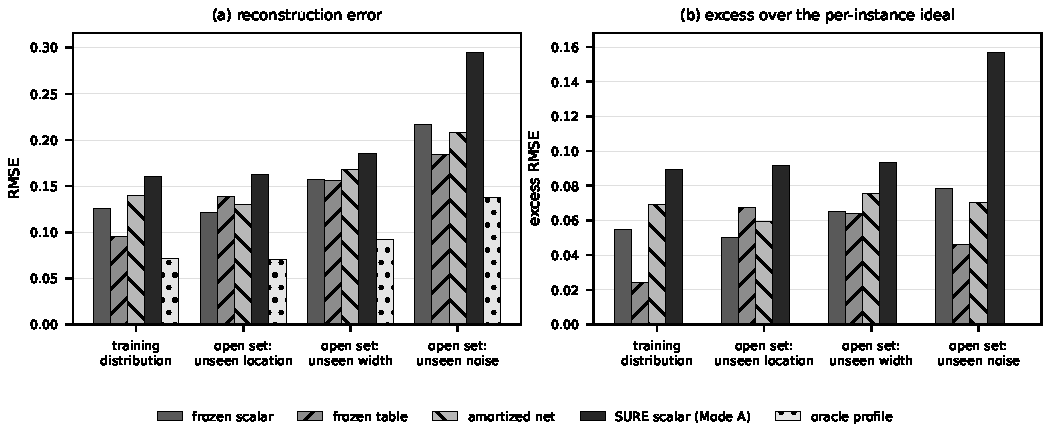
\includegraphics[width=\linewidth]{figures/probe.pdf}
\caption{A minimal empirical probe of the risk gap on a constructed open inversion task, reproduced by \texttt{experiments/probe.py}. Panel (a) reports the reconstruction error of each rule and panel (b) its excess over the per-position ideal of the instance. The corpus-fitted table is the best rule on the training distribution and the only rule within a third of the ideal, and its excess grows by a factor of $1.9$ to $2.8$ on the open set while the ideal is unchanged. Per-instance SURE, the evidence-instantiated rule of the analytic path, and the amortized map do not close the headroom, which is the cost side recorded in Section~\ref{sec:cost}.}
\label{fig:probe}
\end{figure}

\subsection{Relation to Uncertainty Quantification}

Bayesian deep learning distinguishes two kinds of uncertainty: data uncertainty comes from observation noise, and epistemic uncertainty comes from ignorance of model parameters, the latter decreasing as training data grows \citep{kendall2017}. This distinction happens to illuminate the decision axis brightly. Epistemic uncertainty is the statistical representation of Mode B's source of values: parameters are uncertain because their values are determined by a finite corpus, and a different sampling of the corpus gives different values. Mode A rules have no such degree of freedom; camera intrinsics do not change because a thousand more images are captured. Epistemic uncertainty can be calibrated well on closed benchmarks, but the calibrated benchmark itself remains in-distribution, and on the open set there is no distribution to calibrate against.

\subsection{Clues to Endogenous Mechanisms}

Mode A is not an invention of this paper; it has long-standing counterparts in neuroscience. Predictive coding theories of the visual cortex hold that higher levels keep sending predictions of the input to lower levels, which only pass back prediction errors \citep{rao1999}; the free-energy principle describes perception as a whole as the inversion of a generative model \citep{friston2009,friston2010}, with systematic tutorials on its implementation details \citep{bogacz2017}. The common form of these theories is exactly Paradigm I: context rules are endogenous to a single generative objective, and the values of predictions are computed online from current evidence rather than looked up from a frozen parameter table. This paper does not claim that these theories can be copied directly into engineering; it points out only one thing: the inference architecture selected by natural evolution falls on the Mode A side of the decision axis, which is consistent in direction with the negation conclusion of this paper.

\subsection{Existence and Cost of Mode A}
\label{sec:cost}

Whether Mode A really exists determines the practical reading of this paper's conclusion. Existence is substantiated along two paths. The first is the analytic-invariant path: calibrated intrinsics, geometric computations, and coupling strengths solved online from current observations have values given directly by evidence and calibration, bypassing the corpus. The second is the per-instance optimization path: test-time optimization and online inversion solve the rule values separately for each input \citep{sun2020}, and transductive learning is its precedent under near-distribution conditions \citep{vapnik1995}. Predictive coding provides a third clue, already seen in the previous section. Within the range where Assumption A0 holds, Mode A is therefore not an empty class, and the practical reading of this paper's falsification is: a fixed-memory component alone cannot be complete, and a combination with Mode A mechanisms can be complete. On tasks where A0 fails, no mechanism is complete, but they remain within the reach of the negation: Mode B fails there too, except that no Mode A mechanism can take over either.

The cost must be stated plainly. The cost of the analytic-invariant path is constant to linear and negligible. The cost of the per-instance optimization path is about $10^2$ to $10^3$ times one forward computation and is the main bottleneck of real-time systems. The iterative inference path lies in between, depending on the number of iterations needed for convergence. The temptation of Mode B comes exactly from this cost difference: replacing one optimization with one forward pass. The engineering motivation for composite systems lies here too: use Mode B in cost-sensitive and in-distribution stages, and use Mode A in the critical stage of rule generation.

\subsection{Correspondence with Adaptive Control and Online Optimization}

The decision axis has a parallel in control theory. Gain-scheduled control requires the scheduling variables to be measurable and exogenous, with controller parameters looked up or computed from the current operating condition; this is exactly the control-theoretic form of ``rule values instantiated by current evidence'' \citep{shamma1990}; auto-tuning and model-reference adaptive control go further, letting the control law be generated online \citep{astrom1995}. Conversely, an offline-tuned fixed gain table is the control-theoretic embodiment of Mode B, and gain scheduling working by a fixed schedule table is exactly the control-theoretic version of the ``move one level up'' mechanism of the reach section: the schedule table itself is still given by offline experience. Algorithms in online convex optimization that update decisions along the current loss sequence likewise belong to the Mode A side \citep{hazan2016}. The difference is equally worth writing down: online tuning of control laws is guaranteed by Lyapunov stability theory, whereas the correctness of Mode A inference currently has no corresponding stability theory; this is an open problem and the main theoretical gap in the engineering of Mode A.

\subsection{Abstention and the Composite Path}

Two alternative paths need a direct response. The first is detect-and-abstain: the component is highly accurate in-distribution, and it detects anomalies out-of-distribution and refuses to answer. An abstention mechanism decomposes the task into answering and refusing, but completeness requires correct answers on all inputs, and an abstaining system still faces the same decision axis on the inputs it does not refuse; if the refusal rule itself is carried by fixed parameters, detection fails on the open set as well, and the known difficulties of out-of-distribution detection are documented in the literature \citep{hendrycks2016}. Abstention therefore does not escape the decision axis; it merely moves the failure from the answering stage to the detection stage. Abstention is not a dead end: when the refusal criterion is instantiated by evidence, the system can fall back to a search path guided by the measurement model, confining the failure to the detection stage.

The second is composite systems: fixed-memory components propose candidates and likelihoods, Mode A mechanisms generate rules from current evidence, and the arbitration stage controls complexity on near-tree substructures. The limitations section gives necessary-condition-level guidance for composite systems, and one positive sentence is added here: in the legitimate form of a composite system, the credit for completeness goes to the Mode A mechanism, and the Mode B components in it still earn their keep, which is consistent with this paper's delimitation of the weak claim. This also answers the question that engineering practitioners care most about: existing end-to-end systems remain legitimate in-distribution, and what needs to be added is the Mode A loop of rule generation.

\subsection{Design Implications}

Rewrite the decision axis as three engineering questions for system design. First, where do the rule's values come from: corpus statistics, manual setting, current evidence, or analytic calibration. Second, are these values frozen at inference time: frozen is Mode B, and online instantiation is Mode A. Third, on the open set, who is responsible for instantiating the rule: if no mechanism is responsible, the system does not possess completeness for open inversion tasks. The minimal legitimate composite form is therefore: Mode B components provide candidates and likelihoods, a Mode A mechanism generates the rules, and the arbitration stage runs on near-tree substructures. The three questions correspond respectively to the operational readings of Definition~3, Proposition 4, and Theorem 5; the reverse direction, deciding the mode of an implementation that already exists, is the procedure of Section~\ref{sec:procedure}.

\subsection{Limitations}

This paper has four limitations. First, the satisfiability of Criterion P4 is a load-bearing empirical question, and Section~\ref{sec:p4} states the criterion in two components: tasks whose demand can be exactly identified from a fixed corpus fail the barrier condition, and tasks whose fine-scale demand reversals are rare fail the realization condition. In both cases the task is outside the class and a fixed-memory component can be complete, the linear-demand example of Section~\ref{ch:intro} marking the first boundary. No magnitude claim is made: what the barrier-to-gap proposition gives is the floor $\kappa$ of \eqref{eq:floor}, a positive constant attached to the task rather than an unbounded gap. The positive claims additionally need Assumption A0, and tasks whose demand depends on unobserved structure with no trace in the evidence do not satisfy A0, so no mechanism is complete there. Second, the falsification targets ``solo use is complete''; for composite systems it gives only necessary-condition-level guidance and design implications: any fixed-memory component appearing in a combination still has its rules in Mode B, and for a composite system to be complete, some other Mode A mechanism must be present, but this paper gives no sufficient conditions for composite systems. Third, the machine verification covers the carrier-independent algebraic core and the structured general forms, and the remaining modeling components are only the four items listed explicitly in Section~\ref{ch:verify}. Fourth, on the concrete implementation of Mode A, namely how to engineer context rules to be instantiated on the spot by current evidence, this paper gives existence paths and cost magnitudes but no construction scheme; this is the direction of future work. Empirical quantification likewise belongs to future work, with the probe of Section~\ref{sec:probe} standing as a first measurement on a constructed task: what remains is the same comparison of fixed, amortized, and per-instance rule families on a standardized benchmark such as \citep{leuschner2021}, contrasted with data-consistent frozen baselines, together with estimating the barrier separation and the realization level of a concrete task; this paper makes no experimental commitment about the open set of a real deployment.
